\documentclass[12pt, a4paper]{article}

\usepackage[utf8]{inputenc}

% Limit the page margin to only 1 inch.
\usepackage[margin=1in]{geometry}

%Imports biblatex package
\usepackage[
backend=biber,
style=alphabetic
]{biblatex}
\addbibresource{../math-342w.bib}

% Enables the `align' environment.
\usepackage{amsmath}
\usepackage{bm}
\usepackage{array}

% Provides useful environments, such as:
% - \begin{proof} ...\end{proof}
\usepackage{amsthm}
\newtheorem{proposition}{Proposition}
\theoremstyle{definition}
\newtheorem*{definition}{Definition}
\newtheorem{theorem}{Theorem}
\newtheorem{corollary}{Corollary}

% Enables using \mathbb{}, for example \mathbb{N} for the set of natural numbers.
\usepackage{amssymb}

% Allows using letters in enumerate list environment. Use, for example:
%\begin{enumerate}[label=(\alph*)]
% ...
%\end{enumerate}
\usepackage[inline]{enumitem}

% Enable importing external graphic files and provides useful commands, like \graphicspath{}
\usepackage{graphicx}
% Images are located in a directory called "images" in the current directory.
\graphicspath{{./images/}}

% Make links look better by default.
% See: https://tex.stackexchange.com/questions/823/remove-ugly-borders-around-clickable-cross-references-and-hyperlinks
\usepackage[hidelinks]{hyperref}
\usepackage{xcolor}
\hypersetup{
	colorlinks,
	linkcolor={red!50!black},
	citecolor={blue!50!black},
	urlcolor={blue!80!black}
}

% Code Listings. Source:
% https://stackoverflow.com/questions/3175105/inserting-code-in-this-latex-document-with-indentation
\usepackage{listings}
\usepackage{color}
\usepackage[most]{tcolorbox}

\definecolor{dkgreen}{rgb}{0,0.6,0}
\definecolor{gray}{rgb}{0.5,0.5,0.5}
\definecolor{mauve}{rgb}{0.58,0,0.82}

\lstset{frame=tb,
	language=Java,
	aboveskip=3mm,
	belowskip=3mm,
	showstringspaces=false,
	columns=flexible,
	basicstyle={\small\ttfamily},
	numbers=none,
	numberstyle=\tiny\color{gray},
	keywordstyle=\color{blue},
	commentstyle=\color{dkgreen},
	stringstyle=\color{mauve},
	breaklines=true,
	breakatwhitespace=true,
	tabsize=3
}

\newcommand{\prob}{\text{P}}
%\newcommand{\complement}{\mathsf{c}}
\title{Lecture 13: MATH 342W: Introduction to Data Science and Machine Learning}
\author{Sergio E. Garcia Tapia\thanks{Based on lectures of Dr. Adam Kapelner at Queens College.
See also the \href{https://github.com/kapelner/QC_MATH_342W_Spring_2025}{course GitHub page}.}}
\date{March 25, 2025 (last updated \today)}

\begin{document}
	\maketitle
	\section*{Different Modeling Settings}
	We have explored a variety of modeling approaches in the context of
	different response spaces $\mathcal{Y}$. The table below shows some of these:
	\begin{center}
		\begin{tabular}{p{0.2\linewidth}|p{0.2\linewidth}|p{0.2\linewidth}|p{0.3\linewidth}}
			\textbf{Response Space} $\mathcal{Y}$ & \textbf{Output of $g$ belongs to } &
			\textbf{Name} & \textbf{Example Algorithm $\mathcal{A}$}\\
			\hline
			$\mathbb{R}$ & $\mathbb{R}$ & Regression & OLS\\
			\hline
			$\{0,1\}$ & $\{0,1\}$ & Binary Classification & Perceptron, SVM, KNN\\
			\hline
			$\{C_1,C_2,\ldots,C_L\}$ (Nominal) & $\{C_1,C_2,\ldots,C_l\}$ (Nominal) & (Multinomial) Classification & KNN\\
			\hline
			$\{0,1\}$ & $[0,1]$ & Probability Estimation & Logistic Regression
		\end{tabular}
	\end{center}
	Beyond these, the following are discussed in 343:
	\begin{center}
		\begin{tabular}{p{0.2\linewidth}|p{0.2\linewidth}|p{0.2\linewidth}|p{0.3\linewidth}}
			\textbf{Response Space} $\mathcal{Y}$ & \textbf{Output of $g$ belongs to } &
			\textbf{Name} & \textbf{Example Algorithm $\mathcal{A}$}\\
			\hline
			$(0,\infty)$ & $(0,\infty)$ & Survival Modeling & Weibull Regression\\
			\hline
			$\{C_1,C_2,\ldots,C_L\}$ (Nominal) & $\bm{p}$ of dimension $L$ & Probability Estimation & Multilogit Regression\\
			\hline
			$\{0,1,2,\ldots\}$ & $\{0,1,2,\ldots\}$ & Count Modeling & Poisson/Negative Binomial Regression
		\end{tabular}
	\end{center}
	Even beyond the data science course sequence at QC:
	\begin{center}
		\begin{tabular}{p{0.2\linewidth}|p{0.2\linewidth}|p{0.2\linewidth}|p{0.3\linewidth}}
			\textbf{Response Space} $\mathcal{Y}$ & \textbf{Output of $g$ belongs to } &
			\textbf{Name} & \textbf{Example Algorithm $\mathcal{A}$}\\
			\hline
			$(0,1)$ & $(0,1)$ & Proportion Modeling & Beta Regression\\
			\hline
			$\{C_1,C_2,\ldots,C_L\}$ & $\bm{p}$ of dimension $L$ & Ordinal Modeling & Proportional Odds Regression
		\end{tabular}
	\end{center}
	\section*{Probability Estimation}
	Notice that in most models we surveyed, the response space $\mathcal{Y}=\{0,1\}$ was identical
	to the output space of the prediction function $g$. In the table above, however,
	the entry for \textbf{logistic regression} is not like the others: $\mathcal{Y}=\{0,1\}$
	and $g$ returns a number in the interval $[0,1]$. The model function $g$ returns an
	\textit{estimate} of $P(Y=1)$, the probability that the random variable $Y=1$. In this setting,
	the null model $g_0$ is given by:
	\begin{align*}
		g_0 = \bar{y} = \text{the proportion of $1$'s in the $n$ observations
			in our data set $\mathbb{D}$}
	\end{align*}
	Instead of considering $y=t(z_1,\ldots,z_t)$, we consider
	$Y\sim \text{Bernoulli}(t(z_1,\ldots,z_t))$, which is \textit{not} random.
	As usual, we do not know $t$ or the drivers $z_1,\ldots,z_t$, so we use the proxies
	$x_1,\ldots,x_p$. Thus $y$ becomes random. Let
	\begin{align*}
		f_{pr}:\mathbb{R}^{p+1}\to (0, 1)
	\end{align*}
	That is, $f_{pr}$, which is a function of the features, is a probability function.
	Realistically, we are never entirely sure if $y=1$ or $y=0$ (they are degenerate probabilities),
	so we omit them from the co-domain. We approximate $Y$ as
	\begin{align*}
		Y \sim \text{Bernoulli}(f_{pr}(x_1,\ldots,x_p))
	\end{align*}
	which differs based on $\bm{x}$. We can calculate the probability of seeing the historical
	data:
	\begin{align*}
		P(\mathbb{D}) = P(Y_1=y_1, Y_2=y_2,\ldots,Y_n=y_n\mid \bm{x}_1,\bm{x}_2,\ldots,\bm{x}_n)
	\end{align*}
	Assuming that the observations are independent, we can simplify this joint
	probability function into a product of probabilities:
	\begin{align*}
		P(\mathbb{D}) = \prod_{i=1}^{n}P(Y_i=y_i \mid \bm{x}_i)
	\end{align*}
	Recall that if $V\sim \text{Bernoulli}(p)$, then
	\begin{align*}
		P(V = v) = \begin{cases}
			p & \text{if } v = 1\\
			1-  p & \text{if } v = 0\\
			0 & \text{otherwise.}
		\end{cases}
	\end{align*}
	Two other useful ways to write this PMF are:
	\begin{align*}
		P(V=v) = p^v(1-p)^v\quad \text{ and } \quad P(V=v) = pk + (1 - p)(1-k),
	\end{align*}
	where $v\in \{0, 1\}$ (the support of $V$). Then since $Y$ is Bernoulli, we have
	\begin{align*}
		P(\mathbb{D}) = \prod_{i=1}^{n}f_{pr}(\bm{x}_i)^{y_i}(1 - f_{pr}(\bm{x}_i))^{1-y_i}
	\end{align*}
	\section*{Generalized Linear Models}
	Consider an algorithm $\mathcal{A}$ that finds a model by maximizing $P(\mathbb{D})$.
	Similar to before, $f$ is not known; it could be arbitrarily complex. The set of functions
	that map from $\mathbb{R}^{p+1}$ to $(0,1)$ is too large. Thus, let's consider a smaller
	candidate set $\mathcal{H}_{pr}$. As a first attempt, consider again the linear model
	(the set of hyperplanes):
	\begin{align*}
		\mathcal{H}_{pr} = \{\, \bm{w}\cdot \bm{x} \mid \bm{w}\in\mathbb{R}^{p+1}\}
	\end{align*}
	Unfortunately, this does not work because the range of such functions is $\mathbb{R}$,
	and we only want values in the open interval $(0,1)$. We would like to insist on
	a set of candidate functions that retain the linear model $\bm{w}\cdot\bm{x}$
	for the following reasons:
	\begin{enumerate}[label=(\arabic*)]
		\item It is easily interpretable. For example, $b$ is the change in $y$
		if $x_1$ changes by $1$.
		\item Monotone in each feature, making it well-behaved.
	\end{enumerate}
	In order to retain the simplicity of the linear model while still mapping into $(0,1)$,
	we will \textit{transform it}. We need a \textbf{link function}:
	\begin{align*}
		\phi:\mathbb{R}\to (0, 1)
	\end{align*}
	This \textit{links} $\mathbb{R}$ to a different space (i.e., $(0,1)$). There are
	many such functions, but we will restrict our attention to strictly monotonically
	increasing $\phi$. Then the set of candidate functions becomes:
	\begin{align*}
		H_{pr}(\phi) = \{\, \phi(\bm{w}\cdot\bm{x}): \bm{w}\in\mathbb{R}^{p+1}\}
	\end{align*}
	This is the space of \textbf{Generalized Linear Models (GLMs)}. In spite of our
	restriction to monotonically increasing functions, there are still infinitely-many
	link functions. Archetypal examples of link functions include all CDFs of continuous
	random variables whose support is all of $\mathbb{R}$.
	\subsection*{Link Functions}
	The following are examples of link functions, listed in order of popularity:
	\begin{enumerate}[label=(\arabic*)]
		\item \textbf{Logistic}: The logistic (logit, or sigmoid) link function is precisely the
		PDF of the standard logistic random variable:
		\begin{align*}
			\phi(u) = \frac{e^u}{1 + e^u}
		\end{align*}
		Often, we may see it in the following alternate form:
		\begin{align*}
			\phi(u) = \frac{e^u}{1 + e^u}\cdot \frac{e^{-u}}{e^{-u}} = \frac{1}{1 + e^{-u}}
		\end{align*}
		On occasion we will also find it necessary to write:
		\begin{align*}
			1-\phi(u) = \frac{1}{1 + e^{u}}
		\end{align*}
		\item \textbf{Probit}: The probit link function is the CDF of the standard
		normal random variable:
		\begin{align*}
			\phi(u) &= \Phi(u) = \frac{1}{\sqrt{2\pi}} \int_{-\infty}^{v}e^{-v^2/2}\ du\\
			1-\phi(u) &= 1-\Phi(u)=\Phi(-u)
		\end{align*}
		\item \textbf{Cloglog}: Standing for \textit{complementary log-log}, it corresponds to
		the CDF of the standard Gumbel random variable:
		\begin{align*}
			\phi(u) = 1 - e^{-e^u}\iff 1-\phi(u) = e^{-e^u}
		\end{align*}
		Here is a bit of trivia: why is it called complementary log-log? We can see it
		by manipulating the link function:
		\begin{align*}
			\ln(1-\phi(u)) &= -e^u \\
			e^u &= -\ln(1-\phi(u))\\
			u&=\underbrace{\ln(-\ln(\underbrace{1-\phi(u)}_{\text{complement}}))}_{\log\text{-}\log}
		\end{align*}
		\item \textbf{Cauchit}: Corresponds to
		\begin{align*}
			\phi(u) = \frac{1}{\pi} \arctan(u) + \frac{1}{2}
		\end{align*}
		To see that this makes sense, recall that $\lim_{x\to\pm \infty}\arctan(u) = \pm \frac{\pi}{2}$.
		This is known as ``exotic", and is useful when the distribution of $x$'s are very
		variable, (for example, no expectation).
	\end{enumerate}
	The most common are (1) logit and (2) probit.
	\section*{Logistic Regression}
	Let $\phi$ be the logic link, and consider the set of candidate functions
	\begin{align*}
		\mathcal{H}_{pr}(\phi) = \left\{\,
		\frac{1}{1 + e^{-\bm{w}\cdot\bm{x}}} \mid \bm{w}\in \mathbb{R}^{p+1}
		\,\right\}
	\end{align*}
	We further approximate $Y\sim \text{Bernoulli}(h^*_{pr}(x_1,\ldots,x_p))$ (which adds
	misspecification error). Here, $h^*_{pr}(x_1,\ldots,x_p)$ is the best approximation
	of $f_{pr}(x_1,\ldots,x_p)$ in the set $\mathcal{H}_{pr}$. To choose an element
	of $\mathcal{H}_{pr}$ as our $g$, we need an algorithm $\mathcal{A}$, which
	for us will be:
	\begin{align}
		\mathcal{A}:\bm{b}
		= \underset{\bm{w}\in \mathbb{R}^{p+1}}{\text{argmax}}\{\underbrace{P(\mathbb{D})}_{\text{probability}}\}
		\label{eqn:logistic-regression}
	\end{align}
	This algorithm is called \textbf{logistic regression}, and the probability
	on $\mathbb{D}$ s given by
	\begin{align*}
		P(\mathbb{D}) &= \prod_{i=1}^{n}f_{pr}(\bm{x}_i)^{y_i}(1 - f_{pr}(\bm{x}_i))^{1-y_i}\\
		&\approx \prod_{i=1}^{n}\phi(\bm{x}_i)^{y_i}(1 - \phi(\bm{x}_i))^{1-y_i}\\
		&= \prod_{i=1}^{n}\left(\frac{1}{1 + e^{-\bm{w}\cdot \bm{x}_i}}\right)
		\left(\frac{1}{1 + e^{\bm{w}\cdot \bm{x}_i}}\right)^{1-y_i}
	\end{align*}
	When we discussed OLS, we used differentiation to find a vector $\bm{b}$
	that minimized the $SSE$. Can we do something similar to maximize the probability,
	i.e., can we do
	\begin{align*}
		\frac{d}{d\bm{w}}\left(P(\mathbb{D})\right)\stackrel{\text{set}}{=}\bm{0}_{p+1}?
	\end{align*}
	Unfortunately, there are no closed solutions to this as in the OLS case.
	To maximize the probability as specified in Equation~\ref{eqn:logistic-regression},
	we need to use an approximation algorithm. In R, this might involve using
	\texttt{optimx}. The algorithm will yield a feature weight vector $\bm{b}$
	that we can use to define:
	\begin{align*}
		\hat{p} := g_{pr}(\bm{x}) := \phi(\bm{b}\cdot \bm{x}) = \frac{1}{1 + e^{-\bm{b}\cdot \bm{x}}}
		\in (0,1)
	\end{align*}
	The vector $\bm{p}$ is distinct from $\hat{\bm{y}}$, because the latter would be
	a prediction (such as $0$ or $1$ in this the current response space of $\mathcal{Y}=\{0,1\}$),
	whereas $\bm{p}$ is a probability, a real number in $(0,1)$. The probability
	is our guess of $P(Y=1\mid \bm{x})$.
	
	Since we worked hard to retain the linearity in our model (i.e., to retain the
	$\bm{w}\cdot \bm{x}$), let's see how we can use it. We isolate $\bm{b}\cdot\bm{x}$:
	\begin{align}
		\frac{1}{\hat{p}} = 1 + e^{-\bm{b}\cdot \bm{x}}&\iff \nonumber\\
		e^{-\bm{b}\cdot \bm{x}} = \frac{1}{\hat{p}} - 1 = \frac{1-\hat{p}}{\hat{p}} &\iff \nonumber\\
		-\bm{b}\cdot\bm{x} = \ln\left(\frac{1-\hat{p}}{\hat{p}}\right)&\iff \nonumber\\
		\bm{b}\cdot\bm{x} = \ln\left(\frac{\hat{p}}{1-\hat{p}}\right)&
	\end{align}
	The quantity $\frac{\hat{p}}{1 - \hat{p}}\in (0,\infty)$ is called the \textbf{odds of $Y=1$},
	and $\ln\left(\frac{\hat{p}}{1 - \hat{p}}\right)\in \mathbb{R}$ is called the \textbf{log-odds
	of $Y=1$}. Both of these have a one-to-one relationship with $P(Y = 1)$.
	We say that \textit{our model is linear in log-odds}.
	
	What is the relationship between $Y=1$ and $P(Y=1)$? If log-odds is $0$,
	then the probability is $\frac{1}{1 + e^{-0}} = \frac{1}{2}$. The following
	table shows a worthwhile subset of values to be familiar with:
	\begin{center}
		\begin{tabular}{c|c}
			Log-odds & $P(Y=1|\mathbf{x})$\\
			\hline
			$0$ & $\frac{1}{2}$ \\
			$-1$ & $0.27\approx \frac{1}{4}$\\
			$1$ & $0.73\approx \frac{3}{4}$\\
			$-2$ & $0.12\approx \frac{1}{8}$\\
			$2$ & $0.88\approx \frac{7}{8}$\\
			$-3$ & $0.05$\\
			$3$ & $0.95$\\
			$-4$ & $0.02$\\
			$4$ & $0.98$\\
			\hline
			$-\infty$ & $0$\\
			$\infty$ & $1$
		\end{tabular}
	\end{center}
	See also Figure~\ref{fig:log-odds-probability-plot}.
	\begin{figure}
		\centering
		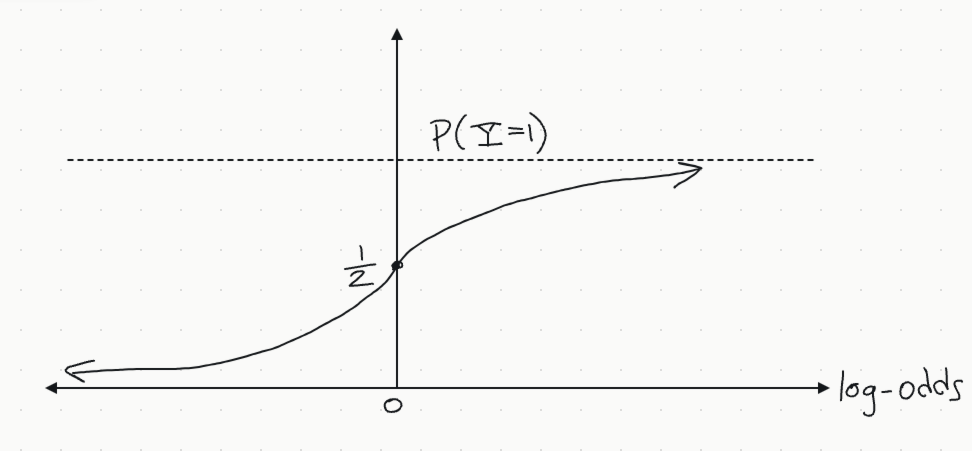
\includegraphics[width=0.7\textwidth]{log-odds-probability-plot}
		\caption{A plot of log-odds versus probability that $Y=1$.}
		\label{fig:log-odds-probability-plot}
	\end{figure}
	Note that depending on the current value of the log-odds, an increase
	by 1 may or may not lead to a substantial increase in probability. For example:
	\begin{itemize}
		\item When the log-odds increases from $0$ to $1$, the probability increases
		from $0.5$ to $0.73$.
		\item When the log-odds increases from $3$ to $4$, the probability increases from
		$0.95$ to $0.98$ (a very small change).
	\end{itemize}
	\section*{Performance Metrics}
	Previously we used $RMSE$ and $R^2$ to assess the predictions of our model.
	For logistic regression, we consider the following \textbf{scoring rules}:
	\begin{enumerate}[label=(\arabic*)]
		\item \textbf{Brier Score}: Let
		\begin{align*}
			s_i := -(y_i - \hat{p}_i)^2
		\end{align*}
		Then the \textit{Brier score} is defined by:
		\begin{align*}
			\bar{s} := \frac{1}{n}\sum_{i=1}^{n}s_i
		\end{align*}
		Note $\bar{s}\leq 0$, since all the $s_i\leq 0$. There are two special cases to consider:
		\begin{itemize}
			\item The \textit{best} Brier score is $0$, when $\hat{p}_i=y_i$
			(that is, the probability is $1$ when the response is $1$, and the probability
			is $0$ when the response is $0$). Then $s_i=0$ for all $i$, and hence
			$\bar{s}=0$.
			\item The \textit{worst} Brier score is $-1$. It occurs when $\hat{p}_i=1-y_i$
			for all $i$, so that $s_i=-1$ for all $i$, and hence $\bar{s}=-1$.
			\item Yet another important case is when $\hat{p}_i = \frac{1}{2}$; the model
			is confused and it becomes a coin toss. In this case,
			\begin{align*}
				\bar{s}=\sum_{i=1}^{n}\left(y_i - \frac{1}{2}\right)^2 = -\frac{1}{4}
			\end{align*}
			In the homework, you will show that the null model $g_0$ beats this Brier score.
		\end{itemize}
		\item \textbf{Log Scoring}: This time, we define
		\begin{align*}
			s_i := y_i\ln(\hat{p}_i) + (1- y_i)\ln(1-\hat{p}_i)
		\end{align*}
		which also satisfies $s_i\leq 0$, since $0<\hat{p}_i<1$ and hence
		both logarithmic expression evaluate to negative. Note that this comes from
		the Bernoulli distribution.
		
		Then the \textit{log scoring rule}
		is given by
		\begin{align*}
			\bar{s} := \frac{1}{n}\sum_{i=1}^{n}s_i
		\end{align*}
		and again we have $\bar{s}\leq 0$. Here, $0$ is best log score value.
		Meanwhile, if $\hat{p}_i=\frac{1}{2}$ for all $i$, we have
		\begin{align*}
			\bar{s} = \frac{1}{n}\sum_{i=1}^{n}\ln\left(\frac{1}{2}\right)=\ln\left(\frac{1}{2}\right)
		\end{align*}
	\end{enumerate}
	\pagebreak
	\printbibliography
\end{document}